\begin{figure*}[!t]
  \centering
        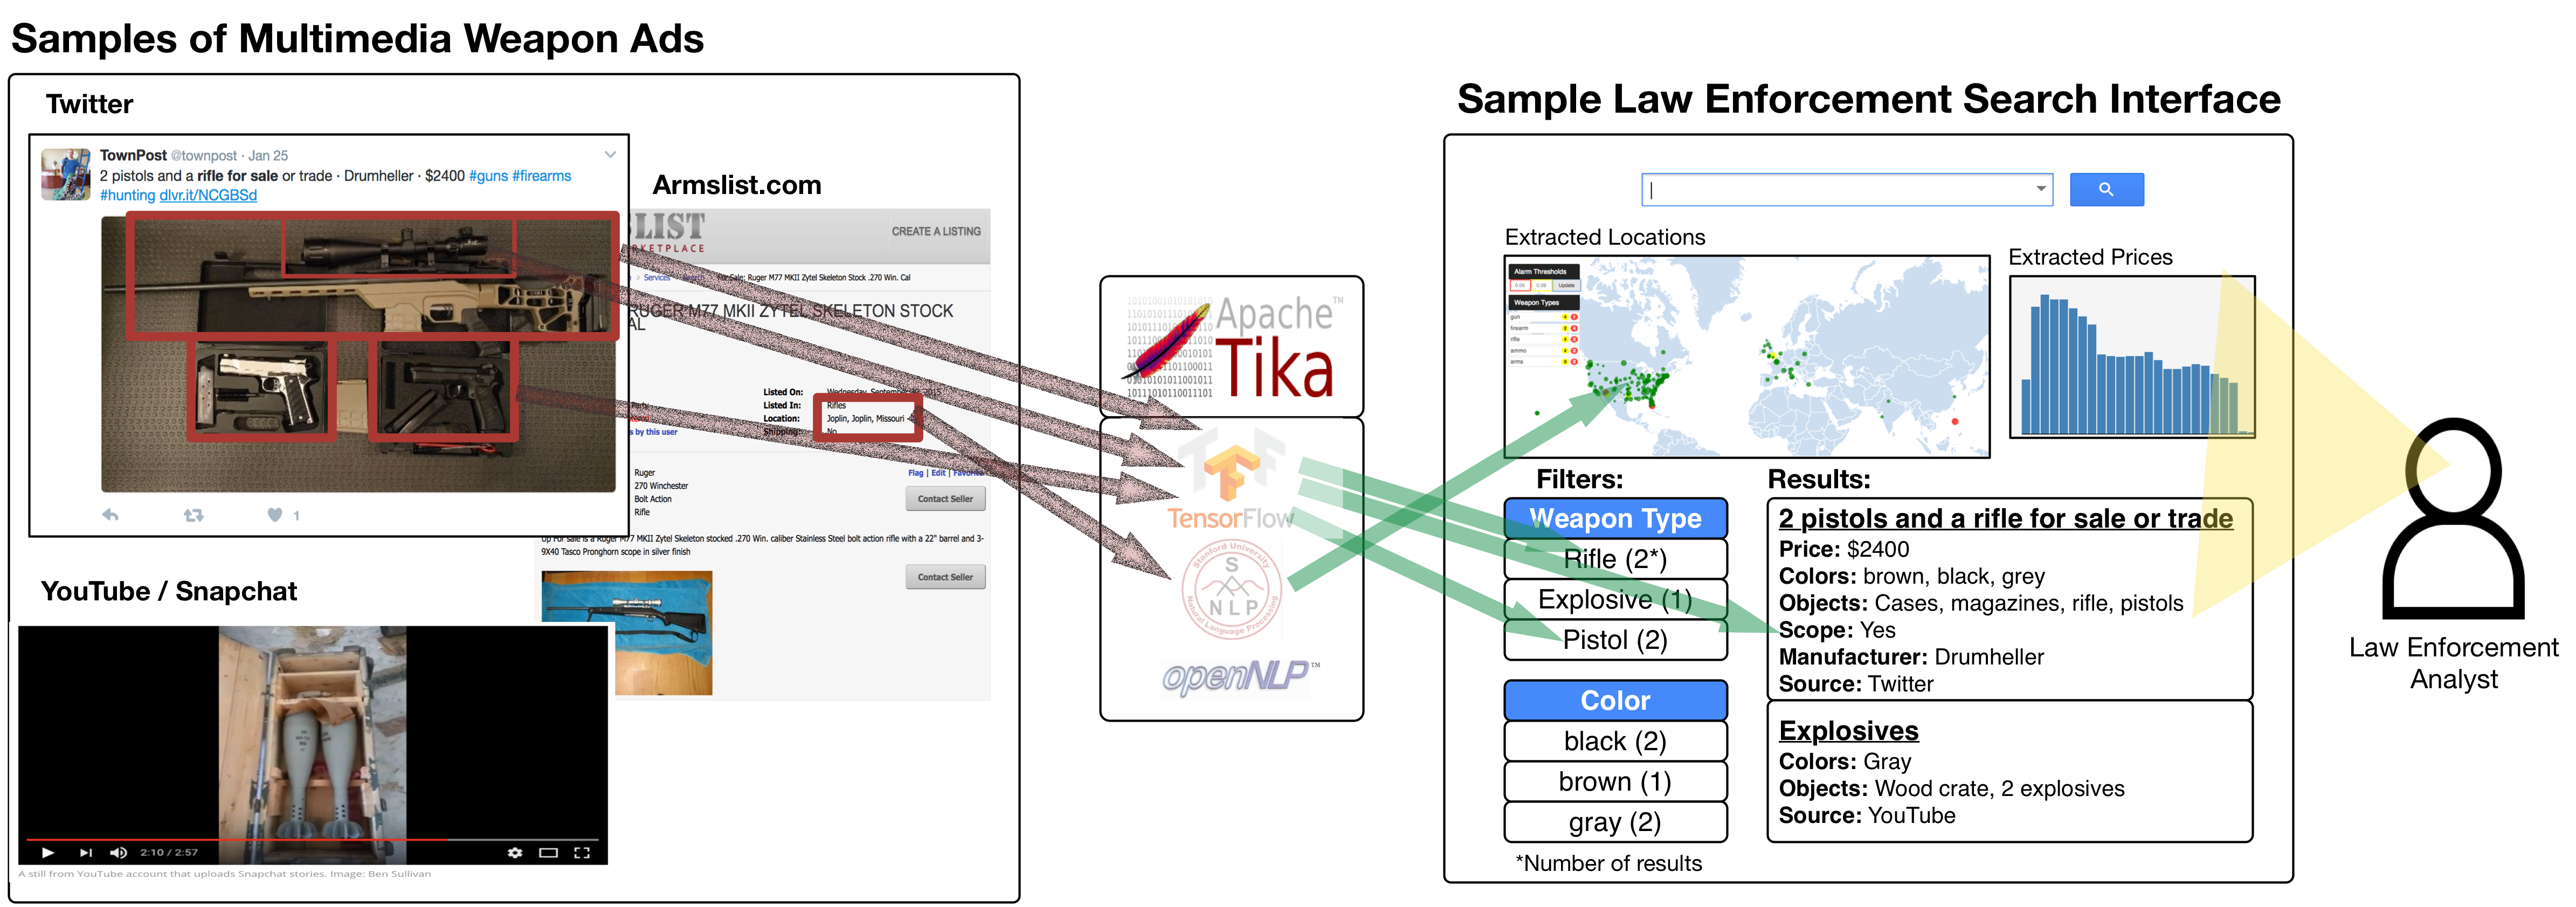
\includegraphics[width=\textwidth,height=6cm]{interface-diagram}
        \caption{This diagram demonstrates how the integration of Tika and Tensorflow facilitates in-depth search across heterogenuous content types. There are several extensions fo our object recognition implementation as well, including more refined categories, optical-character recognition, and image similarity metrics.}
        \label{fig:interface-diagram}
\end{figure*}
\section{INTRODUCTION}
%% TODO: introduce Content Analysis and role in DARPA MEMEX
Over the past two years, our research team has borne witness to the ease and availability of potentially criminal goods and services on the modern Internet. In particular, our team's work on the DARPA Memex project has focused on the issues of online gun sales, as such sales can have grim consequences in that they provide a medium for buyers and sellers to circumvent traditional background checks. In turn, this proliferates the sale of dangerous semi-automatic weapons and can lead directly to loss of human life. For instance, a New York Police Department (NYPD) investigation in 2013 identified guns used in one suicide and four murders and traced their origin to transactions on the website \url{armslist.com}\cite{raja_2016}. 

Unfortunately, law enforcement agencies don't have the manpower to effectively monitor the current scale of online weapons sales. And though the ads, like the whole Internet, contain a large amount of text \cite{mphillips-EOT2012}, the proliferation of images necessitates object recognition and image analysis at scale. Our recent work in DARPA's Memex initiative has expanded Apache Tika, a content detection and analysis framework \cite{mattmann2011tika}, to support such analysis.

The ability to rapidly and automatically detect and analyze gun sales transactions is a significant challenge. There are hundreds of both national and regional gun sales sites like Armslist, \url{floridaguntrader.com}, or \url{gunbroker.com} that share common themes indicative of today's {\em Deep} web. They require a login to either buy or sell, making bulk analysis difficult for traditional web crawlers. A significant number of the sites use AJAX or Javascript for pagination, or for displaying gun images from an ad; this also makes automatic analysis a challenge. Most importantly, the actual content required to answer significant questions regarding these weapons (``is this an automatic weapon?'', ``is this a long or a short gun?'', ``are there multiple weapons being sold?'') are the weapon {\em images} themselves.

We have previously worked on bulk image analysis from the Deep web as it relates to human trafficking data \cite{mattmann7tg} using the Apache Tika. However, that work focused on image metadata forensics as an alternative to image-pixel based analyses and object detection and recognition. Though metadata forensics were promising in human trafficking, weapons required pixel-based analyses. Based on our study of over 80 websites and online forums that specialize in the exchange of weapons, object recognition and computer vision were needed to automatically discern whether or not the guns being sold are automatic or semi-automatic, whether they have been stolen (using serial-number identification), and whether the transactions are potentially illegal. Automatically being able to discern these types of object properties in bulk analyses of image data has the potential to thwart crimes and, ultimately, to save lives.

Historically, the best object recognition systems were inaccurate, but this has changed due to recent advancements in deep neural networks, larger training datasets, and improved computing resources. Tensorflow is a scalable, Python-based system and it natively supports image recognition via its \textit{Inception} model \cite{abadi2016tensorflow}. \textit{Inception} provides a neural network trained on the ImageNet corpus \cite{krizhevsky2012imagenet}, a dataset of 14,197,122 images classified using text from the WordNet taxonomy. The end result is a highly-scalable, off-the-shelf system that can accurately identify and classify objects in images into a thousand categories. This capability -- combined with Apache Tika's native support for detecting thousands of file formats and extracting their metadata and textual content -- is an attractive, automated solution that can perform bulk analysis in the weapons domain, but more generally, in any context where text and images are present and such analyses are required.

Despite its merit, this integration of Tensorflow with Tika presented a significant challenge: Tensorflow does not provide default bindings to Java-based frameworks. Apache Tika is primarily written in Java and thus integrating with Tensorflow is not straightforward like with other JVM-compatible libraries. Our research directly addresses this and contributes several methods that make Tensorflow easier to integrate into Java-based systems like Tika, and any digital forensics system that can make a call to an application programming interface (API). In this paper, we report on our integration of Tika and Tensorflow using the weapons domain as a motivating example. We also evaluate the integration in both its robustness in objection recognition without training beyond that of ImageNet. Lastly, we demonstrate that Tensorflow and Tika together form  a scalable forensics solution for bulk Deep web image analysis.

% The remainder of this paper is organized as follows. Section 2 discusses the collection of the Weapons dataset and its properties. Section 3 presents our integration of Tika and Tensorflow via three methods: (1) command line invocation; (2) Google's RPC (gRPC) integration; and (3) Representational Entity State Transfer (REST) \cite{Fielding:2000:ASD:932295} integration. Section 4 qualitatively and quantitatively evaluates the efficacy of Tensorflow, ImageNet and Tika-based image forensics. Section 5 rounds out the paper.
